\documentclass[]{BasiliskReportMemo}
\usepackage{AVS}


\newcommand{\submiterInstitute}{Autonomous Vehicle Simulation (AVS) Laboratory,\\ University of Colorado}

\newcommand{\ModuleName}{test\textunderscore hingedRigidBodyStateEffector}
\newcommand{\subject}{Integrated test that validates the hinged rigid body state effector}
\newcommand{\status}{Initial document draft}
\newcommand{\preparer}{C. Allard}
\newcommand{\summary}{The hinged rigid body class is an instantiation of the state effector abstract class. This integrated test is validating the interaction between the hinged rigid body module and the rigid body hub that it is attached to. In this case, a hinged rigid body has a diagonal inertia tensor and is attached to the hub by a single degree of freedom torsional hinged with a linear spring constant and linear damping term. The integrated tests has two scenarios it is testing: one with gravity and one without gravity. In both cases orbital energy, orbital momentum, rotational energy, and rotational angular momentum should all be conserved. This integrated test validates for both scenarios that all these paramters are conserved.}


\begin{document}


\makeCover
%
%	enter the revision documentation here
%	to add more lines, copy the table entry and the \hline, and paste after the current entry.
%
\pagestyle{empty}
{\renewcommand{\arraystretch}{1.1}
\noindent
\begin{longtable}{|p{0.5in}|p{4.5in}|p{1.14in}|}
\hline
{\bfseries Rev}: & {\bfseries Change Description} & {\bfseries By} \\
\hline
Draft & Initial document creation & C. Allard \\
\hline

\end{longtable}
}

\newpage
\setcounter{page}{1}
\pagestyle{fancy}

\tableofcontents
~\\ \hrule ~\\



\section{Module Introduction}
The hinged rigid body class is an instantiation of the state effector abstract class. The state effector abstract class is a base class for modules that have dynamic states or degrees of freedom with respect to the rigid body hub. Examples of these would be reaction wheels, variable speed control moment gyroscopes, fuel slosh particles, etc. Since the state effectors are attached to the hub, the state effectors are directly affecting the hub as well as the hub is back affecting the state effectors.

Specifically, a hinged rigid body state effector is a rigid body that has a diagonal inertia with respect to its $\mathcal{S}_i$ frame as seen in Figure~\ref{fig:FlexFigure}. It is attached to the hub through a hinge with a linear torsional spring and linear damping term. The dynamics of this multi-body problem have been derived 

\begin{figure}[htbp]
	\centerline{
		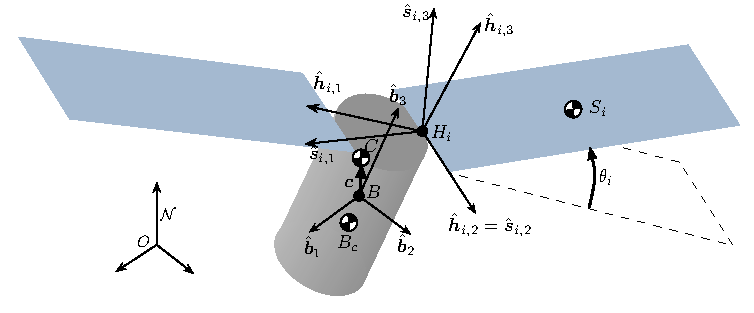
\includegraphics[width=0.8\textwidth]{Figures/Fig4_4_2}}
	\caption{Hinged rigid body frame and variable definitions}
	\label{fig:FlexFigure}
\end{figure}

\section{Module Intended Use}

This module is intended to be used an approximation to a flexing body attached to the spacecraft. Examples include solar arrays, antennas, and other appended bodies that would exhibit flexing behavior. 

\section{Module Assumptions/Limitations}

Below is a summary of the assumptions/limitations:

\begin{itemize}
	\item The hinged rigid body must have a diagonal inertia tensor with respect the $\mathcal{S}_i$ frame as seen in Figure~\ref{fig:FlexFigure}
	\item Only linear spring and linear damping terms
	\item Will only approximate one flexing mode at a time
	\item The hinged rigid will always stay attached to the hub (the hinge does not have torque limits)
	\item The hinge does not have travel limits, therefore if the spring is not stiff enough it will unrealistically travel through bounds such as running into the spacecraft hub
	\item The EOMs are nonlinear equations of motion, therefore there can be inaccuracies that result from integration. Having a time step of $<= 10\ \text{sec}$ is recommended. 
\end{itemize}

\section{Test Description and Success Criteria}

This test is located in \tt SimCode/dynamics/HingedRigidBodies/UnitTest/\newline
test\_hingedRigidBodyStateEffector.py 

\section{Test Parameters}

\section{Test Results}

\input{AutoTex/ChangeInOrbitalAngularMomentumGravity}
\input{AutoTex/ChangeInOrbitalEnergyGravity}
\input{AutoTex/ChangeInRotationalAngularMomentumGravity}
\input{AutoTex/ChangeInRotationalEnergyGravity}

\input{AutoTex/ChangeInOrbitalAngularMomentumNoGravity}
\input{AutoTex/ChangeInOrbitalEnergyNoGravity}
\input{AutoTex/ChangeInRotationalAngularMomentumNoGravity}
\input{AutoTex/ChangeInRotationalEnergyNoGravity}
\input{AutoTex/VelocityOfCenterOfMassNoGravity}
\input{AutoTex/ChangeInVelocityOfCenterOfMassNoGravity}


\end{document}
